
\section{User Interface}
The following section will describe how the Graphical User Interface (GUI) of the Petri net editor, Geometry editor, Appearance editor, Configuration editor and the Simulation tool should look like. How to execute different tasks in the editors such as creating and edit geometry and Petri nets, will be described in the following handbook. The different editors will strive towards being intuitive for the targeted user, e.g. the Geometry editor should be easy for the non-technical user to use, while the Petri net editor should be intuitive for the technical user. 
We are not that far in the actual implementation process to show concrete examples of the GUI. Instead illustrations will be shown of the expected GUI. 

\subsection{Technologies}
The editors will be implemented as extensions to Eclipse, which allows us to use the different functionalities that comes with Eclipse. The functionalities listed below are all part of Eclipse and will be used for this software.

\begin{itemize}
\item{\textbf{Editor:} Used for the Petri net editor and the Geometry editor. Gives the user the ability to create and edit Petri nets and geometries.}
\item{\textbf{View:} Used to show properties of the selected object in the editor and to show the project files.}
\item{\textbf{Dialog:} A pop-up window used when the user has to specify a property of an object or to select textures or 3D files in the Appearance editor.}
\item{\textbf{Wizard:} A pop-up window with several pages that guides the user to fill out information correctly. Used to set up the configuration for the simulator.}
\end{itemize}

The use of these functionalities will all be explained further in the handbook. 

\subsection{Graphical User Interface}
This section will describe the GUI for the editors and the simulation tool. 

\subsubsection{Petri net editor \& Geometry editor}
The Petri net editor and Geometry editor are very much alike. They got the same composition and only the objects that can be drawn on the canvas are different. The Petri net editor and the Geometry editor consist of a toolbar, a view with project files, a view with the properties of the selected object, a canvas and a object toolbar belonging to it. Illustration of the Petri net editor can be seen in figure \ref{fig:petrinet_editor} and an illustration of the Geometry editor can be seen in figure \ref{fig:geometry_editor}. 

\begin{figure}[ht]
	\begin{minipage}[b]{0.45\linewidth}
	\centering
		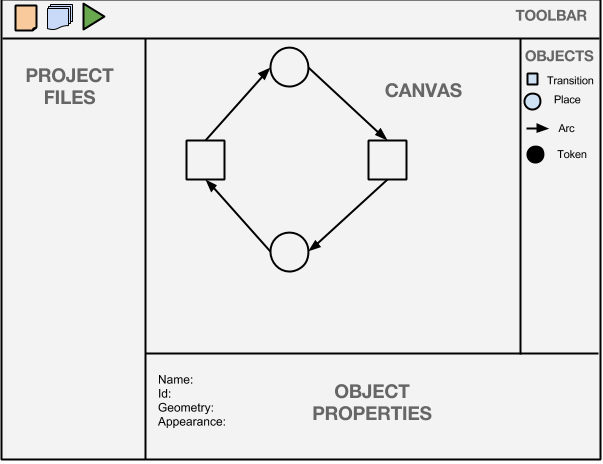
\includegraphics[scale=0.3]{image/petri.png}
\caption{An illustration of the Petri net editor GUI.}
\label{fig:petrinet_editor}
	\end{minipage}
\hspace{0.5cm}
	\begin{minipage}[b]{0.45\linewidth}
	\centering
		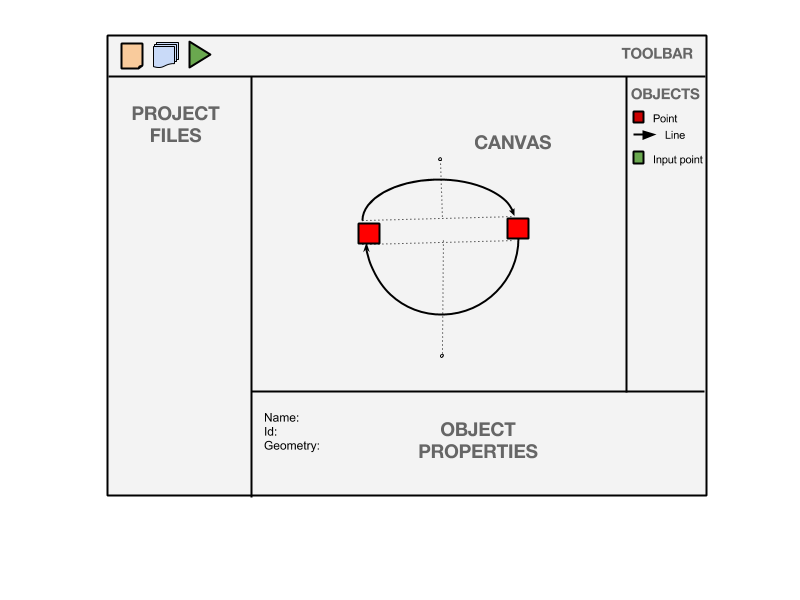
\includegraphics[scale=0.3]{image/geometry.png}
\caption{An illustration of the Geometry editor GUI.}
\label{fig:geometry_editor}
	\end{minipage}

\end{figure}



%\begin{figure}[htp]
%\begin{center}
%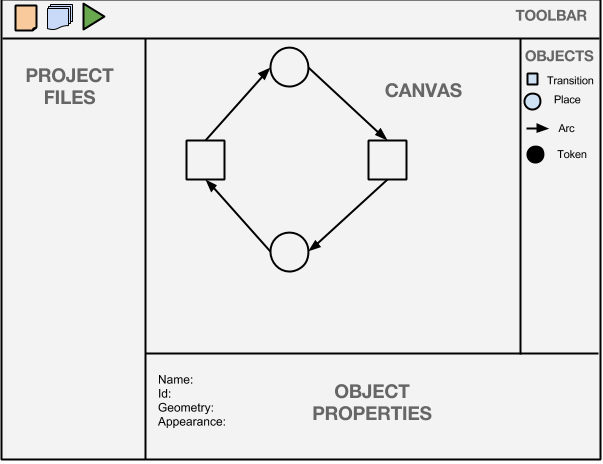
\includegraphics[scale=0.5]{image/petri.png}
%\caption{An illustration of the Petri net editor GUI.}
%\label{fig:petrinet_editor}
%\end{center}
%\end{figure}
%
%
%\begin{figure}[htp]
%\begin{center}
%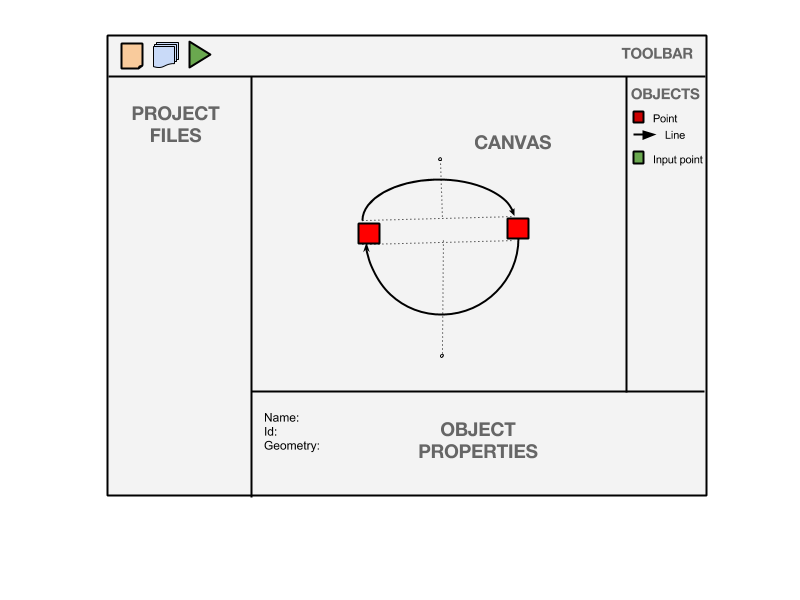
\includegraphics[scale=0.5]{image/geometry.png}
%\caption{An illustration of the Geometry editor GUI.}
%\label{fig:geometry_editor}
%\end{center}
%\end{figure}

\subsubsection{Toolbar}
The toolbar on top allows the user to \textbf{Load} and \textbf{Save} Petri nets as well as Geometries. The \textbf{Play} button allows the user to run the simulation tool anytime he or she wants given that the configuration is set up correctly. 

\subsubsection{Project files}
On the left side the user will have a view where all the files associated to the project are shown. The view will be able to identify the filetype of each file and when the user opens one of the files, the editor associated to the filetype will open accordingly. 

\subsubsection{Canvas}
The canvas will be where the user can draw the Petri net and Geometry respectively. The user drags an object from the Object toolbar and places it on the canvas. The user can edit the position of the different objects by dragging them around on the canvas. Furthermore the connections between the objects can be edited by dragging lines between two objects (while following the rules of the Petri net). The user will be able to see the graphical representation of the Petri net in the Petri net editor and the graphical representation of the geometry in the geometry editor. 

\subsubsection{Objects}
To create and modify the Petri net and the geometry, the user will be able to drag objects from the objects toolbar. The object toolbar in the Petri net editor only has the objects that belongs to Petri net, and the same goes for the geometry editor. As mentioned the user can drag these objects onto the canvas to insert the specific object in the Petri net or geometry. Each object will have a dedicated icon, which will increase usability.

\subsubsection{Object properties}
Each object has different properties that can be defined by the user. The user can modify these properties in the view with the object properties whenever an object is selected. The properties of the different objects in each editor is specified in the System Features. 

\subsubsection{Appearance editor}
Figure \ref{fig:appearance_editor} is an illustration of how the appearance editor will look like. The user has specified in the geometry/petrinet editor the appearance of the object. The appearance can either be a texture to a surface or a 3D object. When the user has specified the appearance with a dedicated label, the user will be able, in the appearance editor, to specify which files should be associated with each label. The user can choose the specific file from the project files.

\begin{figure}[ht]
\begin{center}
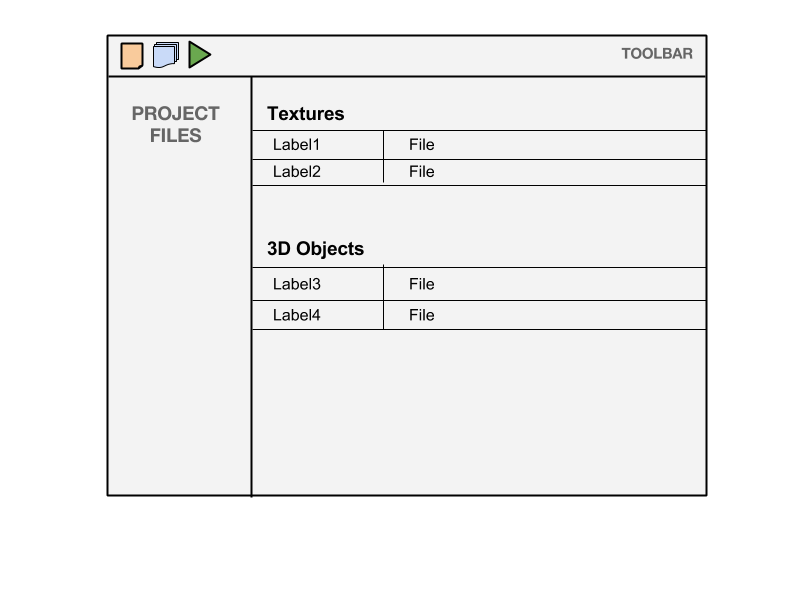
\includegraphics[scale=0.5]{image/appearance.png}
\caption{An illustration of the Appearance editor GUI.}
\label{fig:appearance_editor}
\end{center}
\end{figure}

\subsubsection{Configuration wizard}
The configuration wizard tool helps the user to set up the simulation. The configuration wizard will be a pop-up window with several pages where the user has to specify a file for: Petri net, the geometry and the appearance. The wizard will then validate whether these files match each other. If they do, the user will be able to run the 3D simulation. 

\subsubsection{Simulation tool}
When the user has run the Configuration wizard successfully he will be able to run the 3D simulation. The 3D simulation opens in a new window. This window has a \textbf{play/pause} button that changes according to the play state; if the simulation state is play the button will be a pause symbol and vice versa. The window also has a \textbf{reset} button that allows the user to reset the simulation.
The user will be able to interact with the simulation, therefore the user will be able to use the mouse to click on the different objects the user can interact with. The user will also be able to use the mouse to change the camera perspective.

\begin{figure}[ht]
\begin{center}
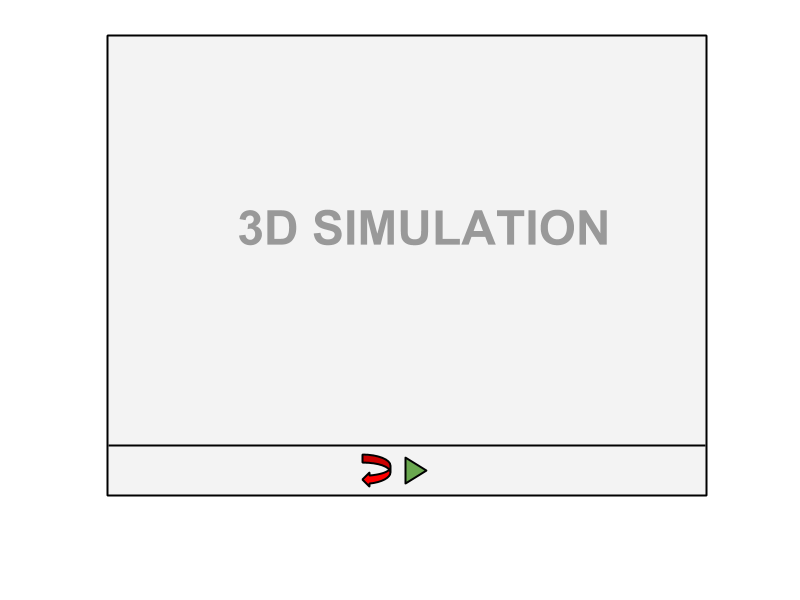
\includegraphics[scale=0.5]{image/simulation_tool.png}
\caption{An illustration of the Simulation tool.}
\label{fig:simulation_tool.}
\end{center}
\end{figure}

\subsection{Handbook}
Since the implementation of this software is only in the beginning stages, the following topics will be an estimation of how the mentioned tasks will be executed. The actual implementation of the software will strive towards being able to do the tasks in this handbook. 
The handbook is a list of typical questions a user will have to the most important parts of this software. A step-by-step guide to solve each of these questions is provided to the reader.

\subsubsection{How do I create a Petri net?}
In the Project files explorer Right-click and choose New $>$ Petri net File ... . \\
A pop-up window will appear where the user can specify the file name. \\
The new Petri net file will appear in the Project files explorer.   

\subsubsection{How do I create a geometry?}
In the Project files explorer Right-click and choose New $>$ Geometry File ... .  \\
A pop-up window will appear where the user can specify the file name. \\
The new geometry file will appear in the Project files explorer.   

\subsubsection{How do add a transition/place to the Petri net?}
Select the transition/place object from the object toolbar on the right. Click and drag the transition/place to the canvas. \\
The transition/place will now appear on the canvas. \\
The user can change the position of the object by click and drag to the new position.

\subsubsection{How do add a point to the geometry?}
Select the point object from the object toolbar on the right. Click and drag the point to the canvas. \\
The point will now appear on the canvas. \\
The user can change the position of the point by click and drag to the new position.

\subsubsection{How do I create a connection between two objects?}
Select the arc/line object from the object toolbar on the right.  \\
Click on the object that is the source and drag the mouse to the target object. \\
The arc/line will now appear on the canvas. 

\subsubsection{How do add a bendpoint to a line?}
Select the line you want to add a bendpoint to. \\
Right-click on the canvas where you want the bendpoint to be and select \textbf{Add bendpoint}. \\
The position of bendpoint can be changed by dragging it with the mouse.

\subsubsection{How do I add an appearance to an object?}
Select an object on the canvas in the Petri net editor / Geometry editor. \\
In the object properties view in the bottom of the editor, change the name in the appearance label for the object. \\
Open the appearance editor. Find the appearance label given in the last step. \\
Click on the \textbf{File..} button next to the label. \\
A pop-up window will appear with a list of the project files. Choose the file you want for the appearance (e.g. a texture file or a 3D object file).\\
When you run the simulation the texture or 3D model will appear for the specific object. 

\subsubsection{How do I delete an object in the Petri net editor and Geometry editor?}
Select and mark the object in the canvas and press Delete.

\subsubsection{How do I save a Petri net model / a geometry model?}
In the editor - click on the \textbf{Save} button in the top toolbar.

\subsubsection{How do I load a Petri net model / a geometry model?}
In the project files explorer - double-click on the model file you want to open. \\
The Petri net editor and geometry editor will open respectively. \\
\newline
The model can also be opened by clicking the \textbf{Load} button in the top toolbar.
A pop-up window will appear with the project files. Select the file you want to open from the list of project files and press Load. 

\subsubsection{How do I run the Configuration wizard?} \label{sec:conf_wizard}
Click on the \textbf{Configuration} button on the top toolbar. 
A pop-up wizard will appear. On the first page in the wizards, select the Petri net file from the project files. On the next page select the geometry model file from the project files. On the third page select the appearance model file. \\
The wizard will now validate whether the 3 files match. If they do the configuration is complete. 

\subsubsection{How do I run the 3D simulation?}
When you have run the Configuration wizard (see steps in section \ref{sec:conf_wizard}) correctly, you will be able to run the simulation. \\
Press the simulation button in top toolbar to run the 3D simulation. 
